
%\section{Question 1}
\textbf{Question:} Simulate the saturation behaviour of a dynamo from helically forced turbulence with forcing wave-number $k_f = 3$ in units of the box wave-number $k_1 = 1$. Use the sample  \texttt{samples/helical-MHDturb}.
\begin{enumerate}
 \item Determine the critical value of the magnetic diffusivity above which there is a growth of the rms magnetic filed, \verb|brms|, in the file \verb|data/time_series.data|
\item Determine the corresponding value of the magnetic Reynolds number, $Re_M = u_{rms}/\eta \kappa_f$
\item Determine the growth rate of the magnetic fiedl for a choseen value of the magnetic diffusivity about half the critical vaule. 
\item Determine the estructure of the magnetic field. Consider the evolution of 3 different magnetic field averages: the \verb|xy| average \verb|bmz|, the \verb|yz| average \verb|bmx| and the \verb|xz| average \verb|bmy|. Run until saturation and determine which of the three averages dominates in the end.
\item Fit the resulting ($\bar{B^2}$) to the expression:
\begin{equation}
 F(t;B_0,t_s)=B_0^2[1-\exp^{-2\eta\kappa_1^2(t-t_s)}]
\label{eq:fitB}
\end{equation}
\end{enumerate}

\subsection{Solution.}

\subsubsection{Critical value for the magnetic diffusivity.}

Calculation of the critical value for the magnetic diffusivity implies running the code for different values of the magnetic diffusivity and checking up at which value the field starts growing.

In figure \ref{fig:brmst} the growth of the rms magnetic field versus time can be analyzed for different magnetic diffusivity values.

\begin{figure}[h]
\centering
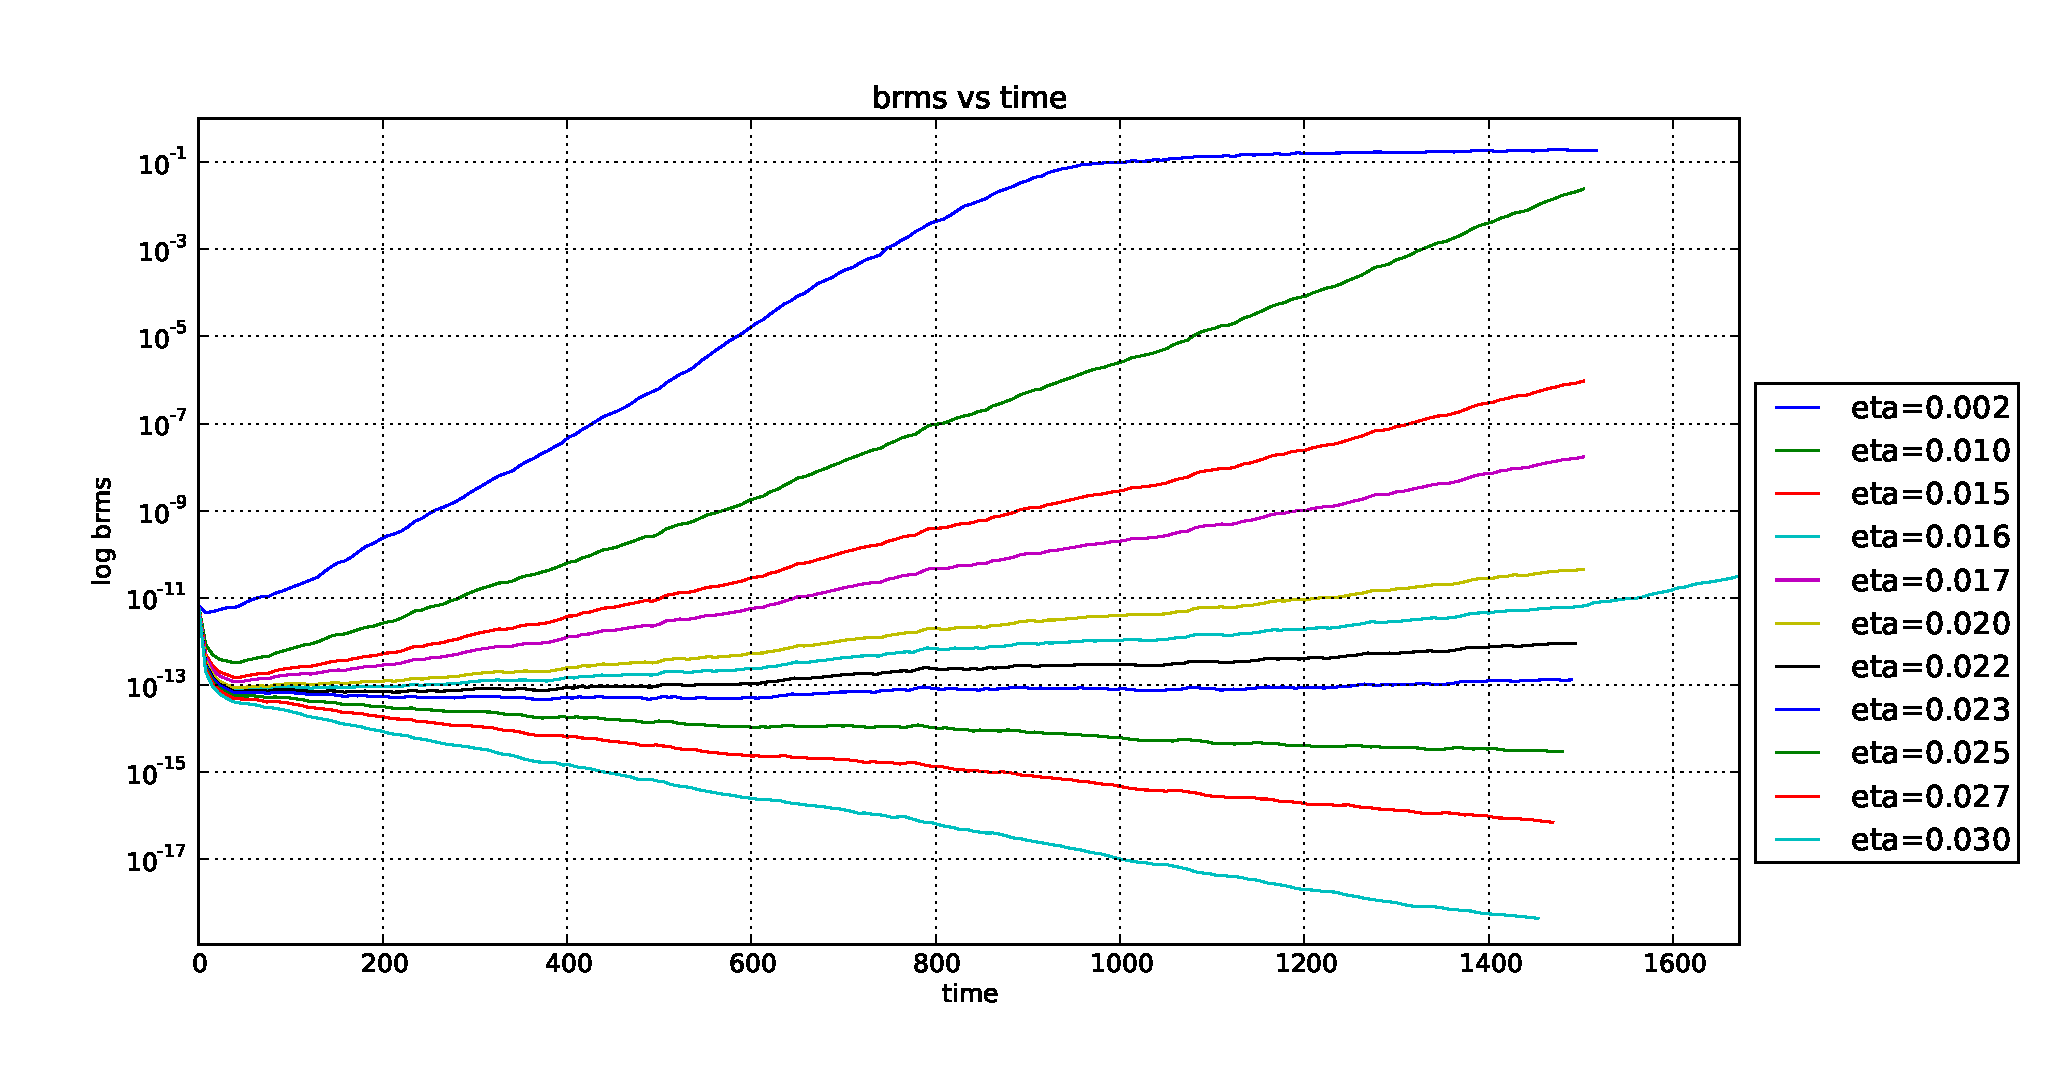
\includegraphics[width=0.7\textwidth]{brms_vs_time.eps}
\caption{log(brms) vs time for different values of  magnetic diffusivity.}
\label{fig:brmst}
 \end{figure}

Using these results, I set the critical value for the magnetic diffusivity in $\eta = 22e-3$.

\subsubsection{Magnetic Reynolds number}
\begin{figure}[h]
\begin{minipage}{.70\textwidth}
The magnetic Reynolds number is defined as:
\begin{equation}
 Re_M = \frac{u_{rms}}{\eta \kappa_f}
\end{equation}
We have set $\kappa_f = 3$, the critical value for the magnetic diffusivity found is  $\eta = 22e-3$ and the mean value for $u_{rms}$ is $\bar{u_{rms}} = 0.14$, so the corresponding magnetic Reynolds number is $Re_M = 2.15$.

The magnetic Reynolds number is the ratio between convection and diffusion. When $Re_M \gg 1$, convection dominates, whereas for $Re_M \approx 1$, or less, diffusion becomes important. So, in this exercise, diffusion is about to become important.

In fact, the table \ref{tab:re}  shows that $Re_M$ decreases as $\eta$ increases
 \end{minipage}
\hspace{0.5cm}
\begin{minipage}{.30\textwidth}
\begin{center}
\begin{tabular}{ll}
$\eta$ & $Re_M$\\\hline
2e-3 & 22.39\\
10e-3 & 4.73\\
15e-3 & 3.16\\
16e-3 & 2.97\\
17e-3 & 2.78\\
20e-3 & 2.37\\
22e-3 & 2.15\\
23e-3 & 2.06\\
25e-3 & 1.89\\
27e-3 & 1.75\\
30e-3 & 1.58\\
\end{tabular}
\label{tab:re}
\end{center}
\end{minipage}
\end{figure}



\subsubsection{Growth rate of the magnetic field}

In order to determine the growth rate of the magnetic field for a value of the magnetic diffusivity, one must fit the sloped part of the logarithm of $brms$ vs time curve, as shown in the figures \ref{fig:growth2} and \ref{fig:growth10}.

\begin{figure}[h]
\begin{minipage}{.45\textwidth}
\centering
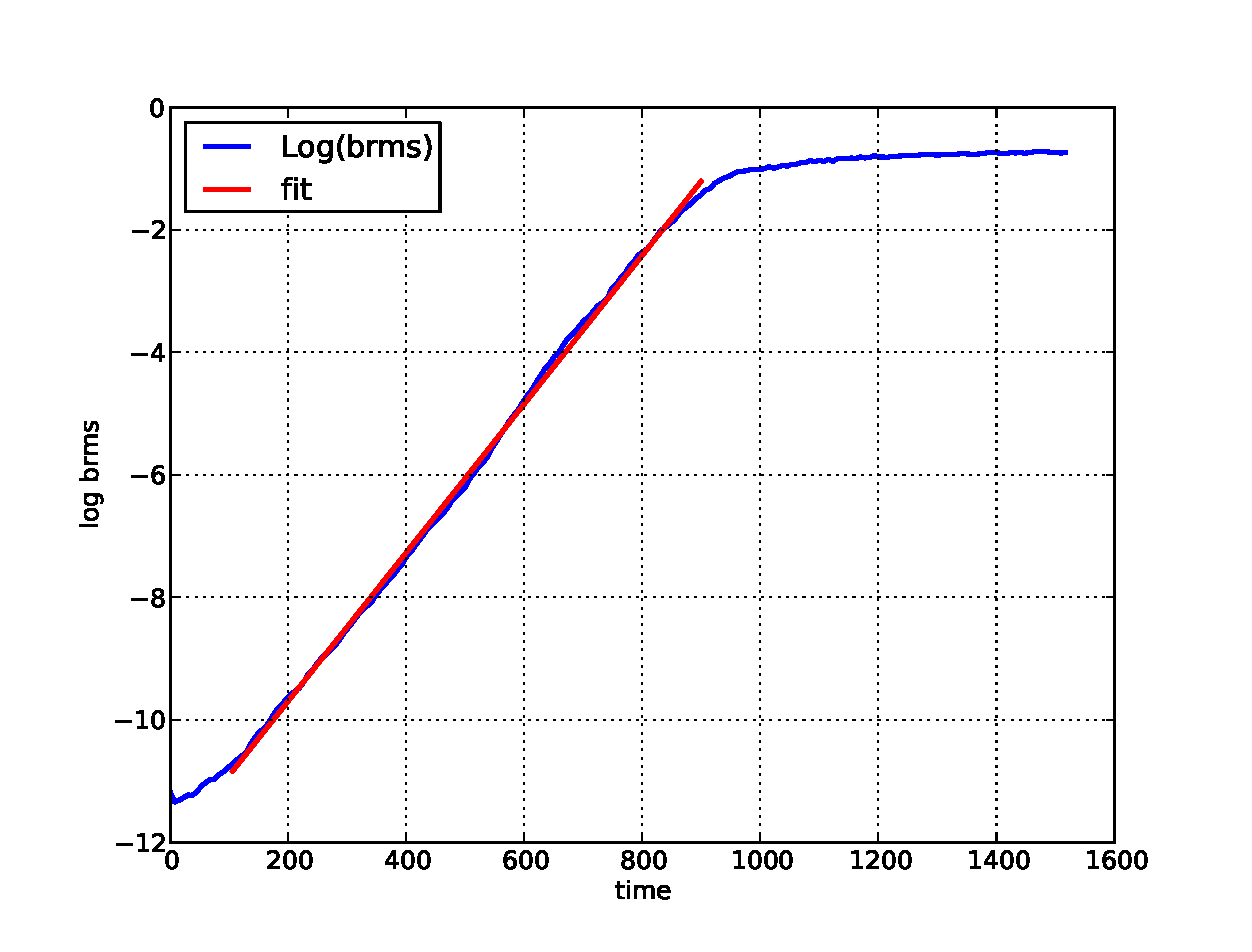
\includegraphics[width=\textwidth]{growth2e-3.eps}
\caption{Growth rate of the magnetic field for a value of the magnetic diffusivity  $\eta = 2e-3$.}
\label{fig:growth2}
\end{minipage}
\hspace{0.5cm}
\begin{minipage}{.45\textwidth}
\centering
 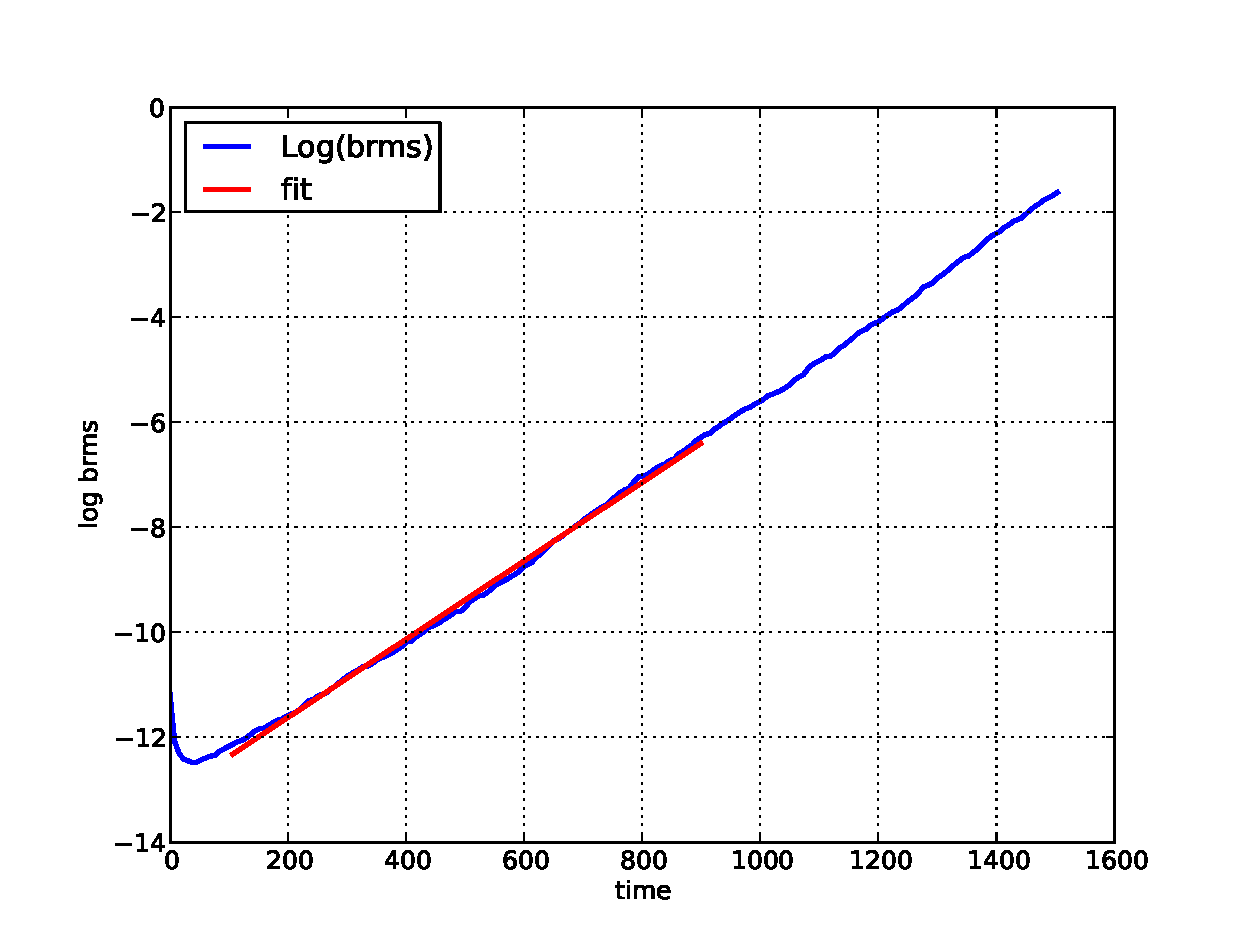
\includegraphics[width=\textwidth]{growth10e-3.eps}
\caption{Growth rate of the magnetic field for a value of the magnetic diffusivity  $\eta = 10e-3$.}
\label{fig:growth10}
\end{minipage}
 \end{figure}
%y=ax+b
The parameter $a$ in a linear regression fit ($y=ax+b$) is a measure of the growth rate of the magnetic field. The growth depends on the value of the magnetic diffusivity, and it decreases as the magnetic diffusivity increases.
\begin{center}
\begin{tabular}{lll}
$\eta$ & a & b\\\hline
2e-3 & 0.0121 & -12.12\\
10e-3 & 0.0075 & -13.11
\end{tabular}
\end{center}

\subsubsection{Structure of the magnetic field.}

\begin{figure}[h]
\begin{minipage}{.45\textwidth}

\centering
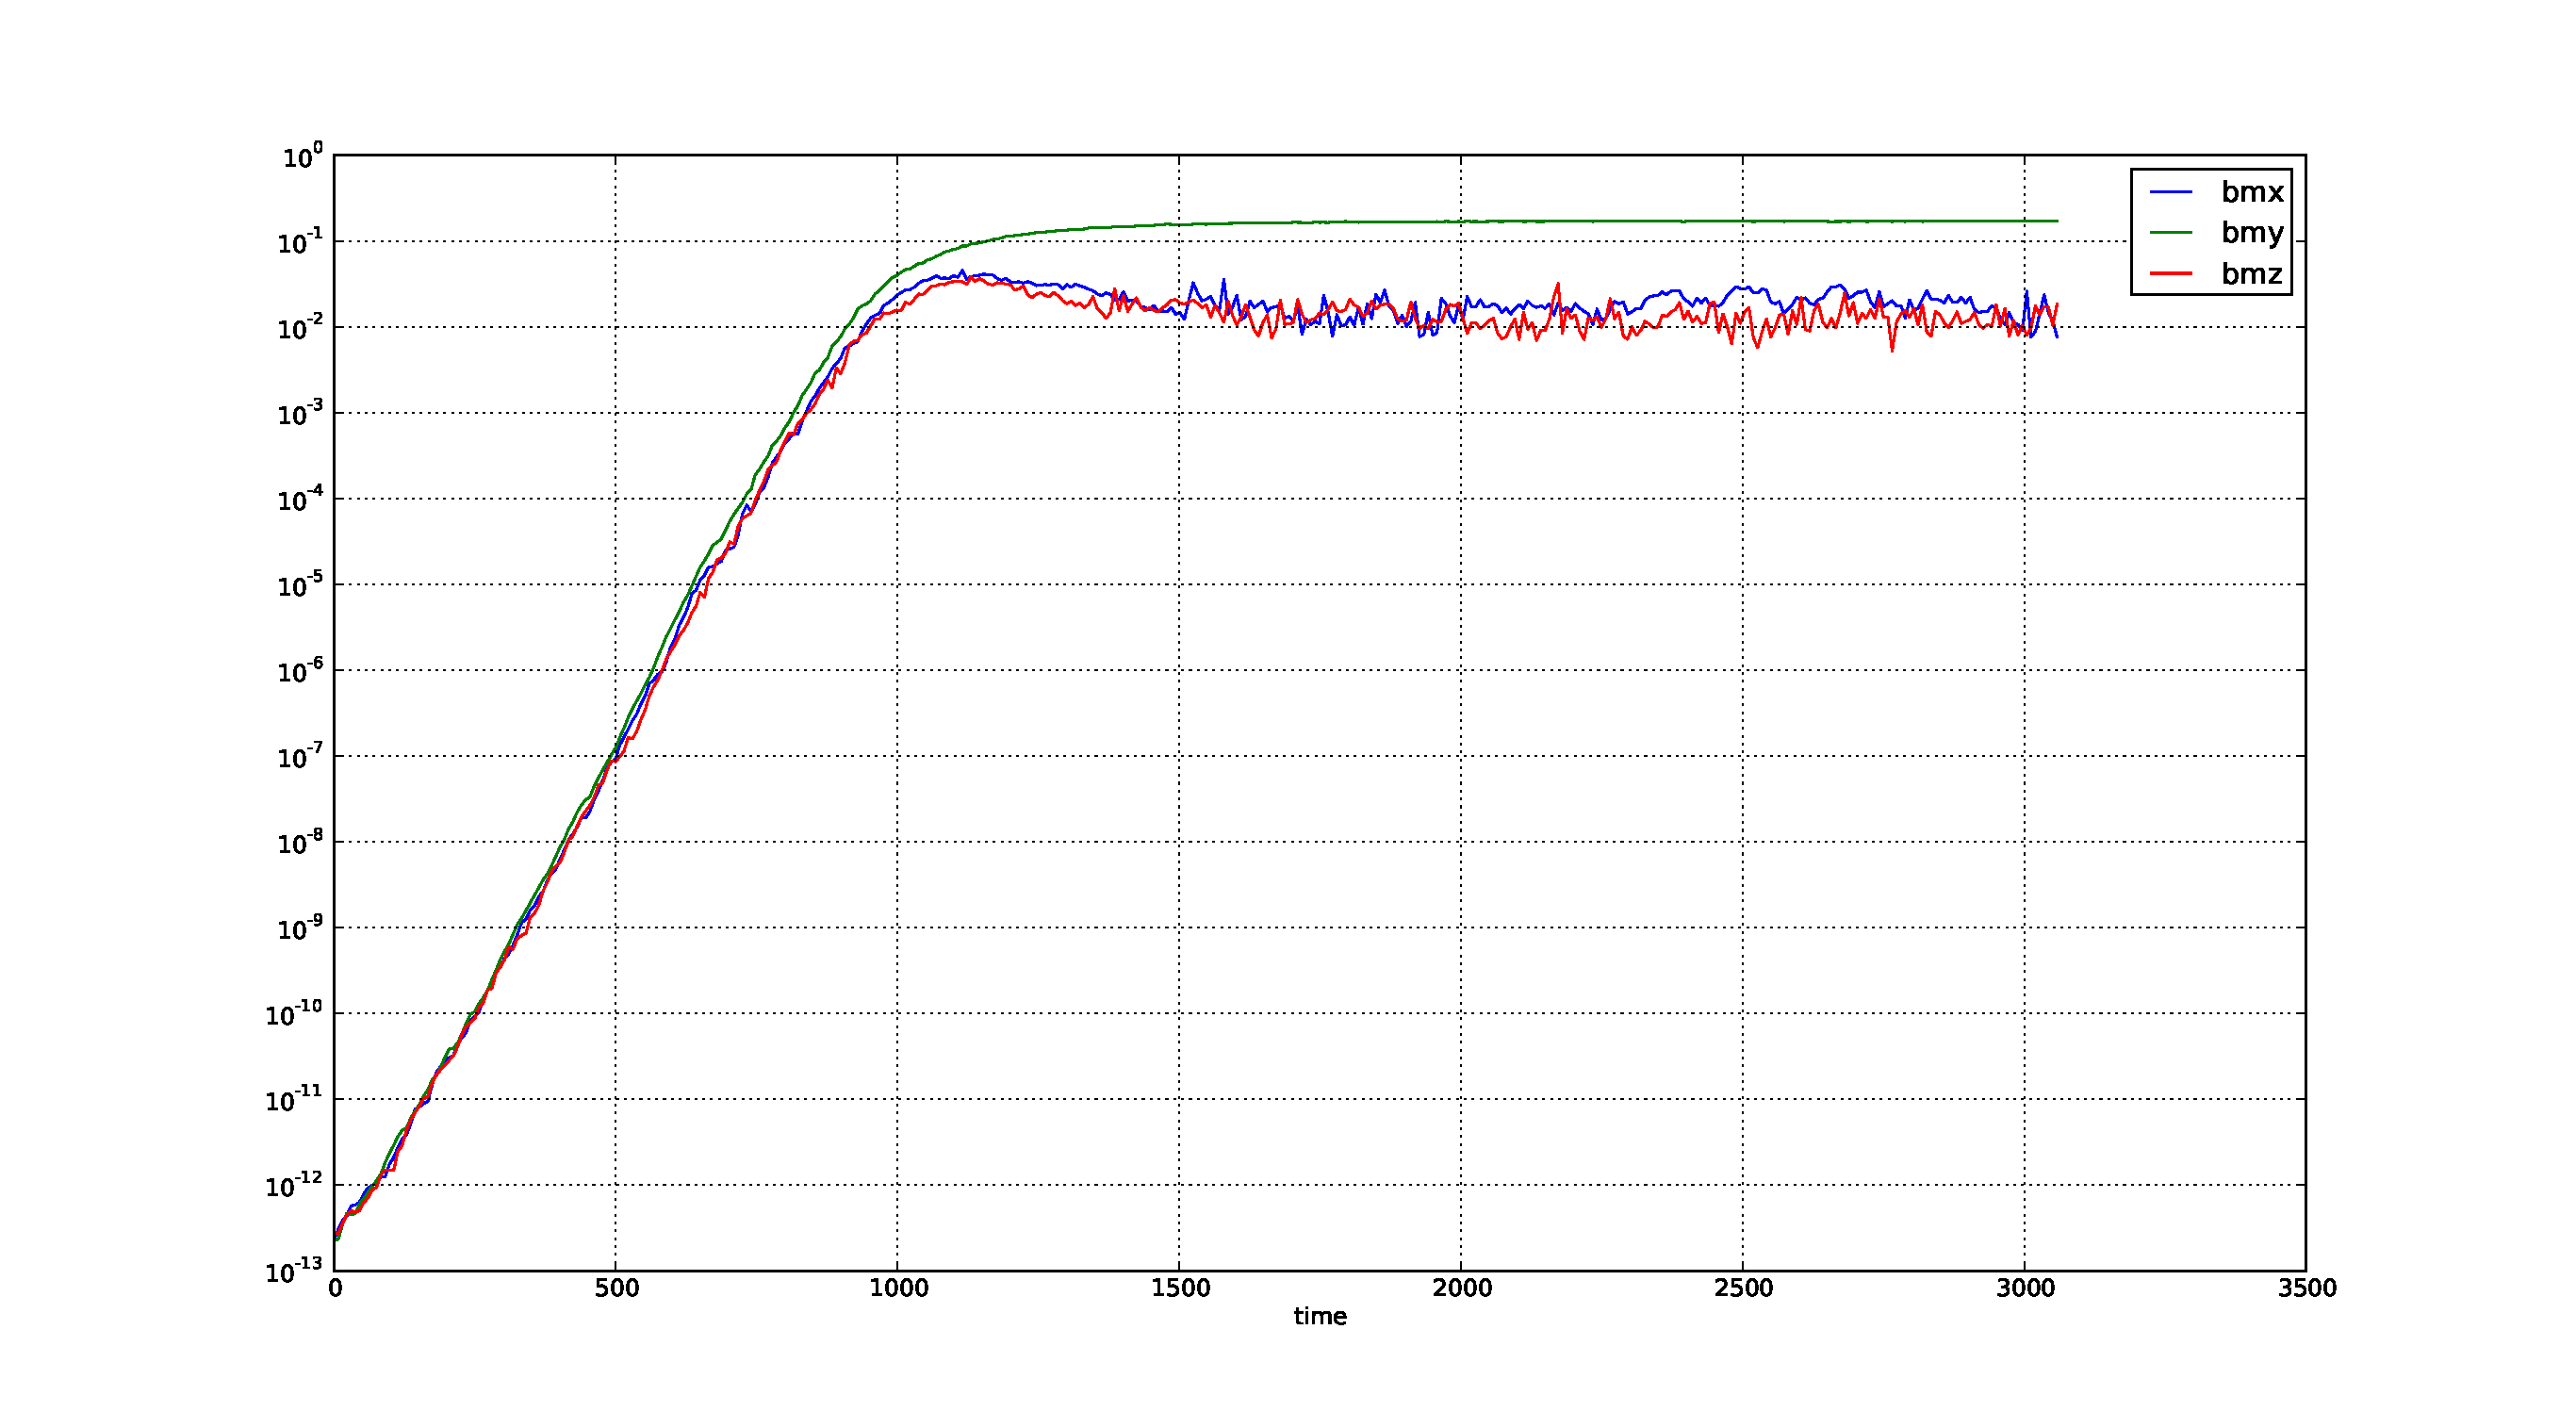
\includegraphics[width=\textwidth]{campos3.eps}
\caption{Averages of three different magnetic fields.}
\label{fig:averages}

\end{minipage}
\hspace{0.5cm}
\begin{minipage}{.45\textwidth}
Figure \ref{fig:averages} shows the evolution of three different magnetic field averages: the xy average bmz, the yz average bmx and the zx average bmy. 
From the figure one can see that the $zx$ average dominates in the end.
\end{minipage}
 \end{figure}

\subsubsection{Fitting $B_{zx}$}
The strongest of the three field averages is the zx average represented in the figure \ref{fig:bmy_fit} with different values of the expression \ref{eq:fitB}.
\begin{figure}[h]
\centering
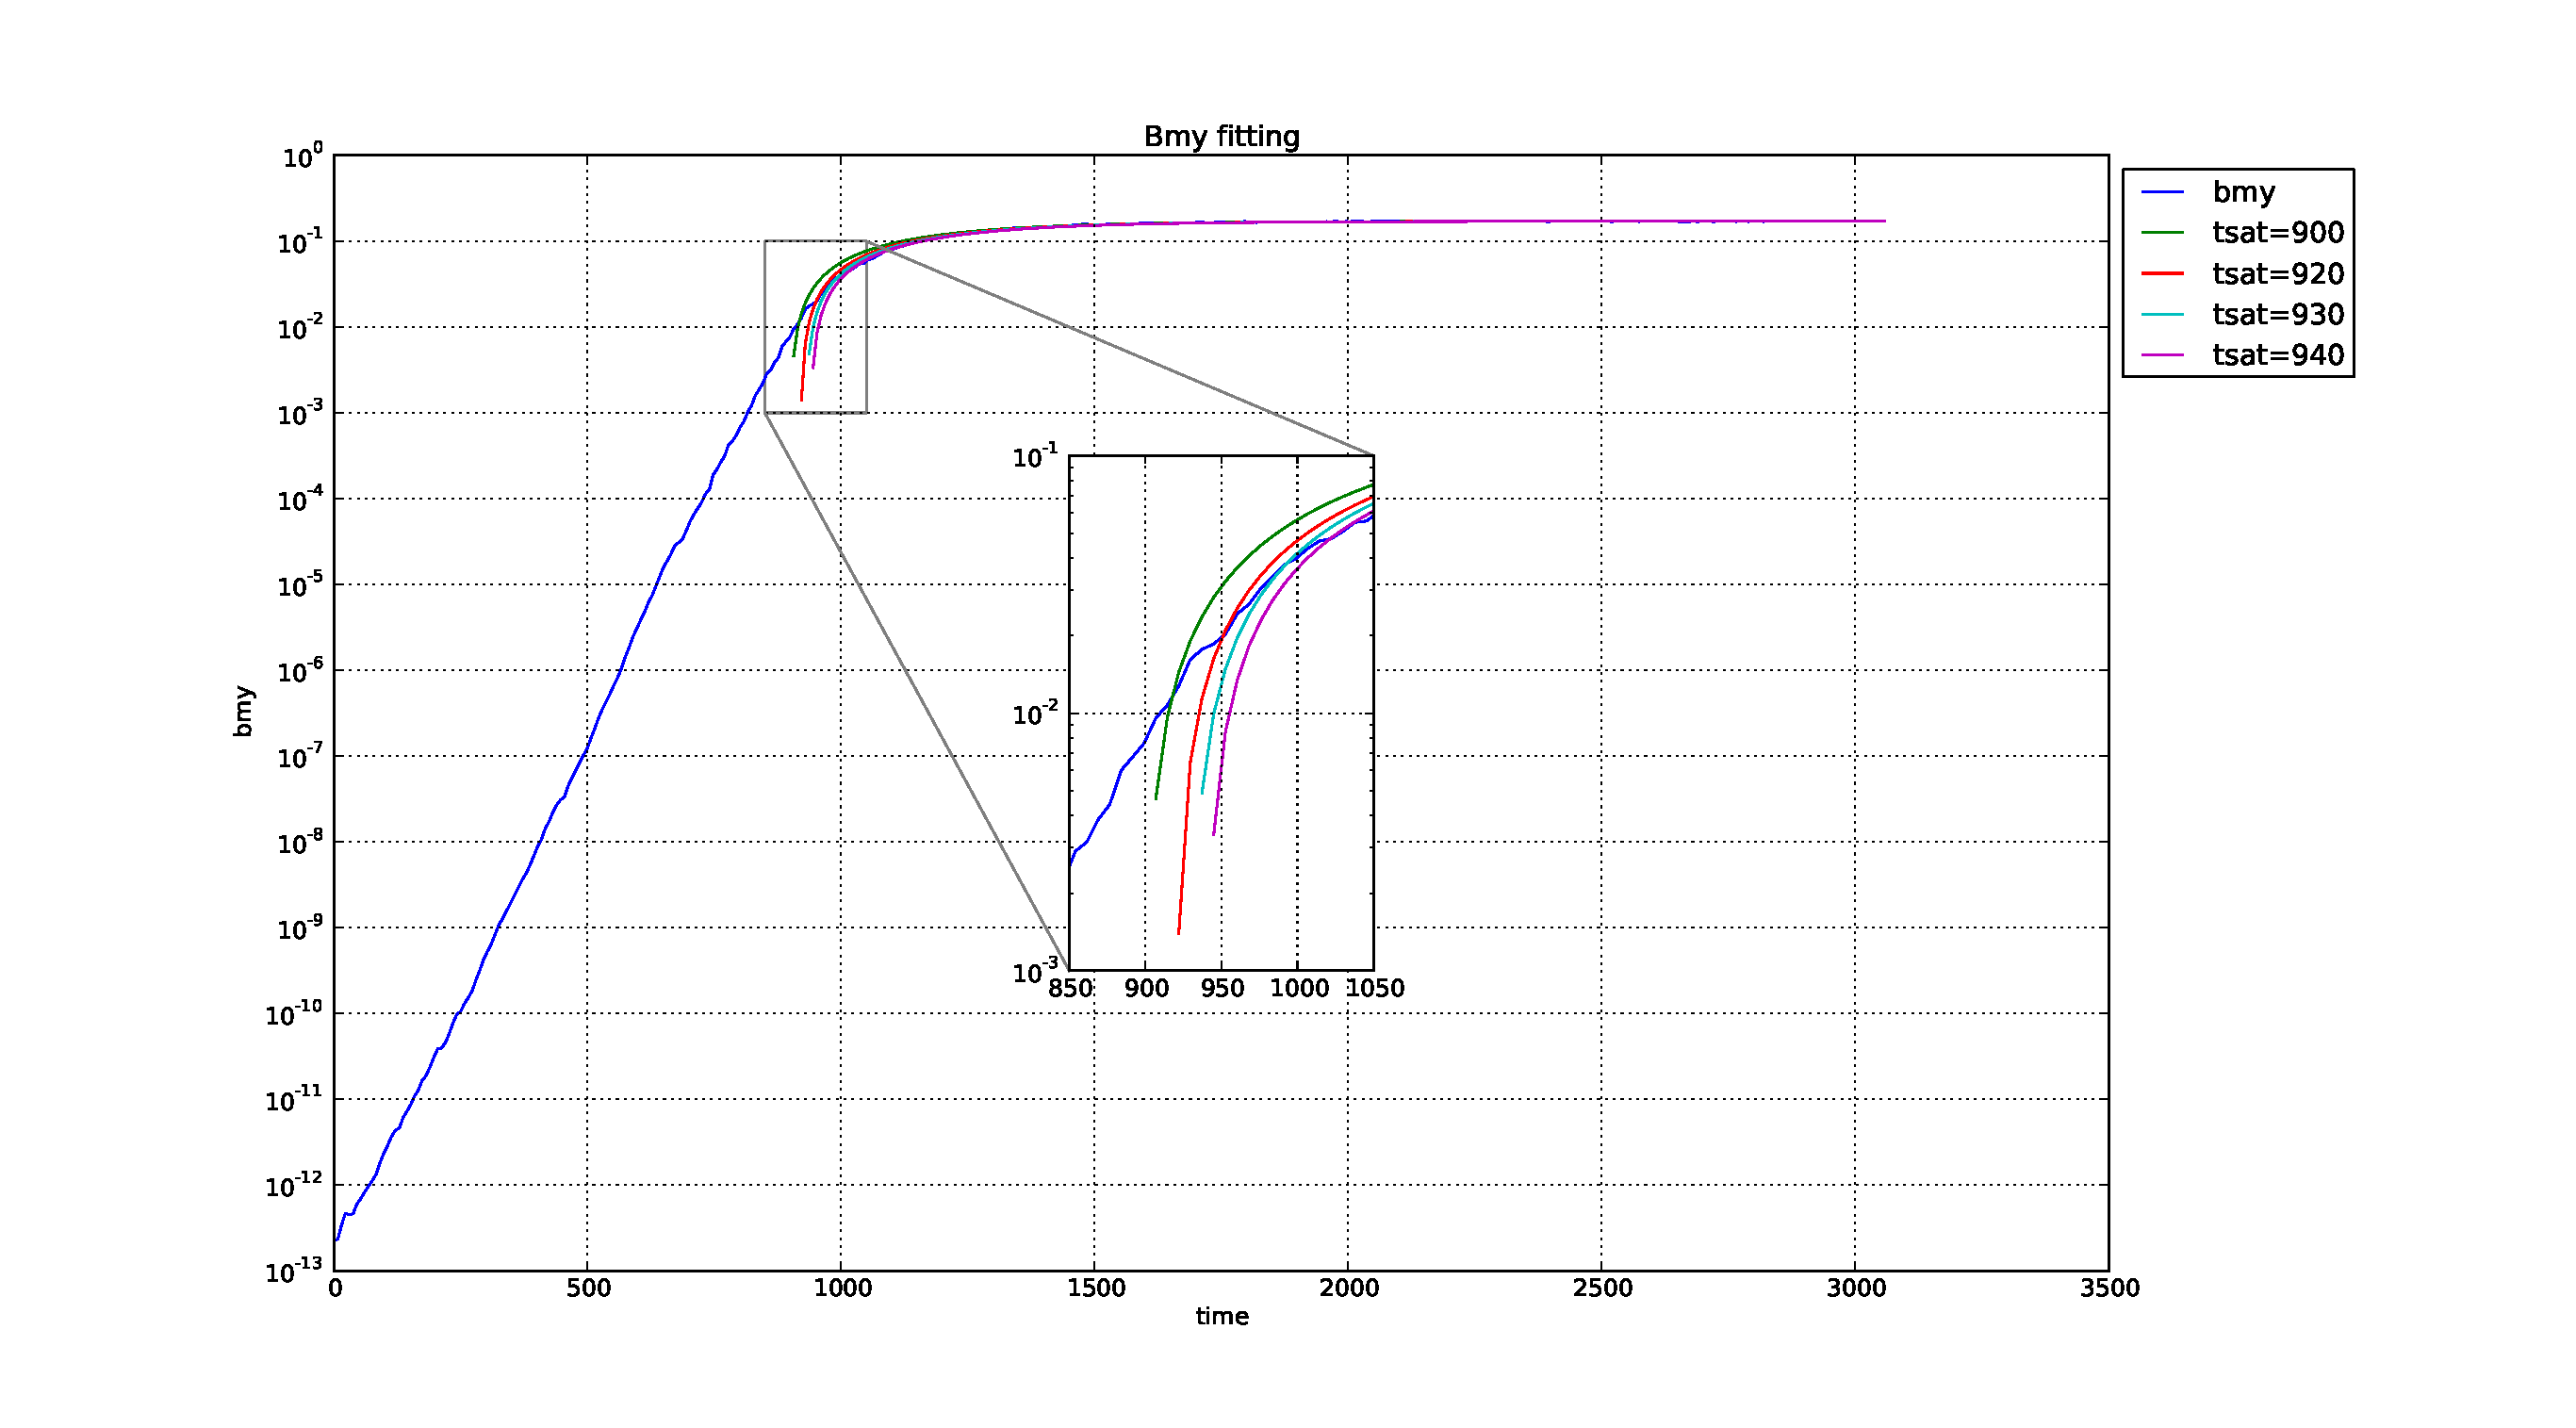
\includegraphics[width=0.8\textwidth]{bmy_fit.eps}
\caption{Bmy Fitting: $B_0=0.1712$ and $t_s = 930$.}
\label{fig:bmy_fit}
 \end{figure}
A rough fit for the field average takes the values $B_0=0.1712$ and $t_s = 930$.
$B_0$ is the saturation field value and $t_s$ is the best fit curve just before saturation.

